A photograph of a newt is shown in Figure \ref{fig:newt}.
\begin{figure}[!h]
    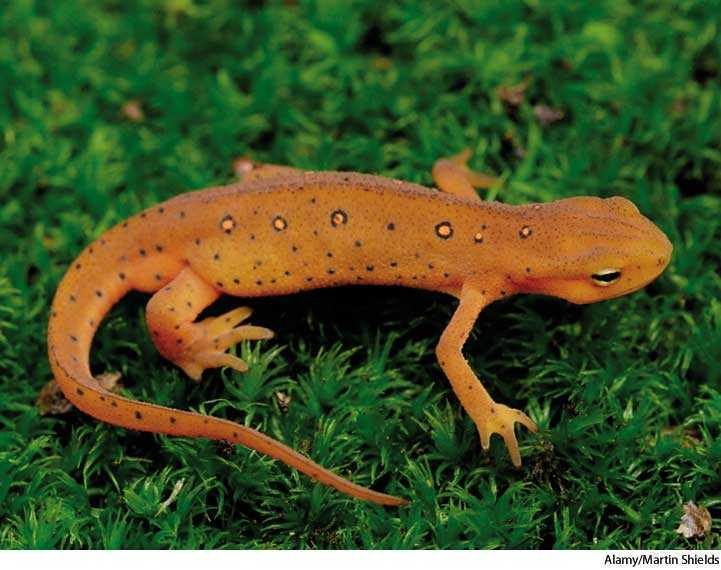
\includegraphics[width=0.95\columnwidth]{newt.jpg}
    \caption{A newt.}
    \label{fig:newt}
\end{figure}

One of the oldest citable scientific papers is \cite{van1677concerning}.

\begin{table}[!htp]
	\normalsize
	\centering
	\caption{Method comparison}
	\begin{tabular}{lcc}
		\toprule
			& Our method & Other methods\\
		\midrule
		Good & \checkmark & \xmark \\
		Bad  & \xmark     & \checkmark
		\bottomrule
		\label{tab:comparison}
	\end{tabular}
\end{table}

In Table \ref{tab:comparison}, we illustrate the value of our method.
